\documentclass{beamer}
\mode<presentation>
{
	\usetheme{Antibes}
}
\usepackage[utf8]{inputenc}
\usepackage[english]{babel}

\usepackage{tikz}
\usetikzlibrary{graphs, positioning, arrows, matrix}
\usepackage{sansmathaccent}
\pdfmapfile{+sansmathaccent.map}
\usepackage{amssymb,latexsym,amsmath,amscd,amsthm, mathtools,stmaryrd, hyperref,array, cleveref}

\title{Supersingular Isogeny Diffie-Hellman}
\author{Valeriia Kulynych}
\institute{Université de Toulon}
\date{May 25th, 2018}
\begin{document}

\begin{frame}
	\titlepage
\end{frame}

\begin{frame}
	\frametitle{Outline}
	\tableofcontents
\end{frame}

\section{Supersingular Elliptic Curves}

\begin{frame}
\frametitle{Elliptic curves}
	\begin{definition}
		An \alert{elliptic curve} is a pair $(E, O)$, where $E$ is a curve of genus 1 and $O \in E$.
	\end{definition}
	\setbeamertemplate{itemize items}[circle]
	\begin{itemize}
		\item We consider curves defined over field $K$ with characteristic $p > 0$.
	
		 \item Composition law is defined as follows:
		Let $P, Q \in E$, $L$ be the line connecting $P$ and $Q$ (tangent line to $E$ if $P = Q$), and $R$ be the third point of intersection of $L$ with $E$. Let $L'$ be the line connecting $R$ and $O$. Then $P \oplus Q$ is the point such that $L'$ intersects $E$ at $R, O \ \text{and} \ P \oplus Q$.
	
	\end{itemize}
	

\end{frame}

\begin{frame}
%\frametitle{Composition Law}
\begin{figure}
	\hfill
	%% 
	\begin{center}
	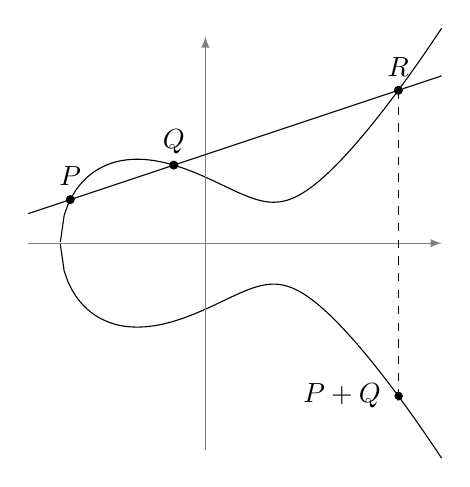
\begin{tikzpicture}[domain=-2.4566:4,samples=100,yscale=3/8,xscale=3/4]
		\draw plot (\x,{sqrt(\x*\x*\x-4*\x+5)});
		\draw plot (\x,{-sqrt(\x*\x*\x-4*\x+5)});
	
		\draw[thin,gray,-latex] (0,-7) -- (0,7);
		\draw[thin,gray,-latex] (-3,0) -- (4,0);
	
		\draw (-3,1) -- (4,8/3+3);
		\begin{scope}[every node/.style={draw,circle,inner sep=1pt,fill},cm={1,2/3,0,0,(0,3)}]
			\node at (-2.287980,0) {};
			\node at (-0.535051,0) {};
			\node at (3.267475,0) {};
		\end{scope}
		\begin{scope}[every node/.style={yshift=0.3cm},cm={1,2/3,0,0,(0,3)}]
			\node at (-2.287980,0) {$P$};
			\node at (-0.535051,0) {$Q$};
			\node at (3.267475,0) {$R$};
		\end{scope}
	
		\draw[dashed] (3.267475,3.267475*2/3+3) -- (3.267475,-3.267475*2/3-3) 
			node[draw,circle,inner sep=1pt,fill] {}
			node[xshift=-0.1cm,anchor=east] {$P+Q$};
	\end{tikzpicture}
	\hfill
	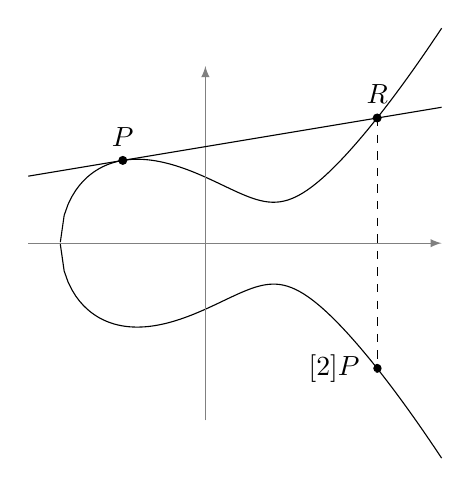
\begin{tikzpicture}[domain=-2.4566:4,samples=100,yscale=3/8,xscale=3/4]
		\draw plot (\x,{sqrt(\x*\x*\x-4*\x+5)});
		\draw plot (\x,{-sqrt(\x*\x*\x-4*\x+5)});
		
		\draw[thin,gray,-latex] (0,-6) -- (0,6);
		\draw[thin,gray,-latex] (-3,0) -- (4,0);
	
		\def\c{3.269524}
		\def\P{-1.398674}
		\def\R{2.908459}
		\draw (-3,-1+\c) -- (4,4/3+\c);
		\begin{scope}[every node/.style={draw,circle,inner sep=1pt,fill}, cm={1,1/3,0,0,(0,3.269524)}]
			\node at (\P,0) {};
			\node at (\R,0) {};
		\end{scope}
		\begin{scope}[every node/.style={yshift=0.3cm},cm={1,1/3,0,0,(0,3.269524)}]
			\node at (\P,0) {$P$};
			\node at (\R,0) {$R$};
		\end{scope}
	
		\draw[dashed] (\R,\R/3+\c) -- (\R,-\R/3-\c) 
			node[draw,circle,inner sep=1pt,fill] {}
			node[xshift=-0.1cm,anchor=east] {$[2]P$};
	\end{tikzpicture}

		\hfill
		\strut
	
	\end{center}
	
	\caption{An elliptic curve defined over $\mathbb{R}$, and the geometric
		representation of its group law.}
	\label{fig:weierstrass}
\end{figure}
\end{frame}

\begin{frame}
\frametitle{Supersingular Elliptic Curves}
	\begin{definition}
		For every $n$, we have a multiplication map 
			\[[n]: E \to E\]
			\[ P \mapsto \underbrace{P \oplus \cdots \oplus P}_{n \ \text{times}}. \]
		Its kernel is denoted by $E[n]$ and is called the $n$-torsion subgroup of $E$. Then one can show that for any $r \geq 1$:
			\[ E[p^r](\bar{K}) \simeq
				\begin{cases}
					{0} \\
					\mathbb{Z}/p^r\mathbb{Z}
				\end{cases} \]
		In the first case, $E$ is called \alert{supersingular}. Otherwise, it is called ordinary.
	\end{definition}
\end{frame}

\section{Isogeny Graphs}

\begin{frame}
\frametitle{Isogenies}
	\begin{definition}
		Let $E_1$ and $E_2$ be elliptic curves defined over a finite field $\mathbb{F}_q$ of characteristic $p$. An \alert{isogeny} $\phi: E_1 \to E_2$ defined over $\mathbb{F}_q$ is a non-constant morphism that maps the identity into the identity (and this a is group homomorphism).
	\end{definition}
	
	\begin{theorem}[Sato-Tate]
		Two elliptic curves $E_1$ and $E_2$ are isogenous over $\mathbb{F}_q$ if and only if $\#E_1(\mathbb{F}_q) = \#E_2(\mathbb{F}_q)$. 
	\end{theorem}

	\begin{itemize}
		\item Curves in the same isogeny class are either all supersingular or all ordinary.
		
		\item The degree of an isogeny $\phi$ is the degree of $\phi$ as a morphism. An isogeny of degree $\ell$ is called $\ell$-isogeny.
	\end{itemize}
\end{frame}

\begin{frame}
\frametitle{Isogeny graphs}

	\begin{definition}
		Let $E$ be an elliptic curve over a field $K$. Let $S \subseteq \mathbb{N}$ be a finite set of primes. Define
			\[X_{E, K, S} \]
		to be the graph with vertex set being the $K$-isogeny class of $E$. Vertices are typically labelled by $j(E)$. There is an edge $(j(E_1), j(E_2))$ labelled by $\ell$ for each equivalence class of $\ell$-isogenies from $E_1$ to $E_2$ defined over $K$ for some $\ell \in S$. This graph is called \alert{isogeny graph}.
	\end{definition}

	Supersingular isogeny graph is always
		\begin{itemize}
			\item conncted;
			\item $\ell + 1$-regular, where $\ell$ is isogeny degree.
		\end{itemize}
\end{frame}

\begin{frame}
\begin{figure}[h]
	\begin{center}
		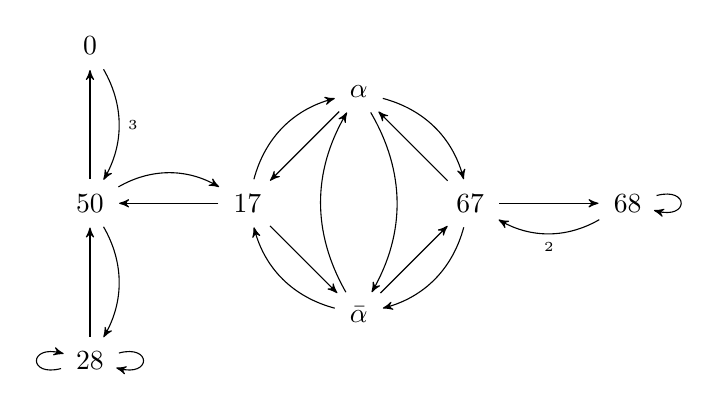
\begin{tikzpicture}[->, shorten >=2pt, shorten <=2pt, >=stealth', node distance = 2cm]
		
		\node (1) {$17$};
		\node (2) [above right of=1] {$\alpha$};
		\node (3) [below right of=1] {$\bar{\alpha}$};
		\node (4) [below right of=2] {$67$};
		\node (5) [right of=4] {$68$};
		\node (6) [left of=1] {$50$};
		\node (7) [below of=6] {$28$};
		\node (8) [above of=6] {$0$};
		
		\path
		(1) edge [bend left] (2)
		(1) edge (3)
		(1) edge (6)
		
		(2) edge (1)
		(2) edge [bend left] (3)
		(2) edge [bend left] (4)
		
		(3) edge [bend left] (1)
		(3) edge [bend left] (2)
		(3) edge (4)
		
		(4) edge (2)
		(4) edge [bend left] (3)
		(4) edge (5)
		
		(5) edge [bend left] node[below]{\tiny{$2$}} (4)
		(5) edge [loop right] (5)
		
		(6) edge [bend left] (1)
		(6) edge [bend left] (7)
		(6) edge (8)
		
		(7) edge (6)
		(7) edge [loop left] (7)
		(7) edge [loop right] (7)
		
		(8) edge [bend left] node[right]{\tiny{$3$}} (6);
		
		\end{tikzpicture}
	\end{center}
	\caption{Supersingular Isogeny Graph $X_{\bar{\mathbb{F}}_{83}, 2}$}\label{SIG83.figure}
\end{figure}

\end{frame}

\begin{frame}
\begin{figure}[h]
	\begin{center}
		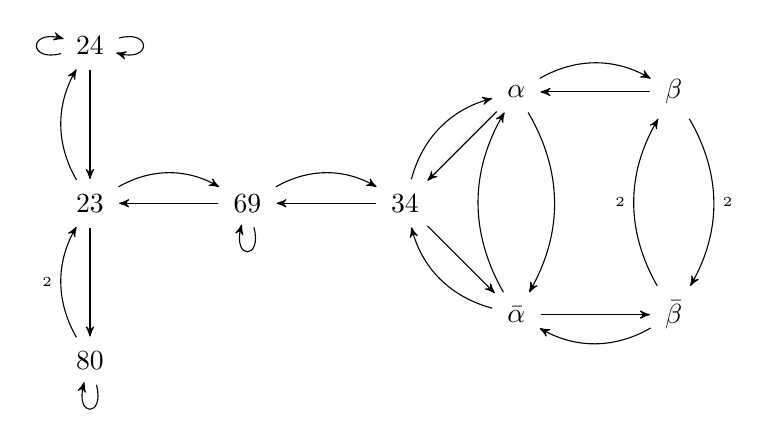
\begin{tikzpicture}[->, shorten >=2pt, shorten <=2pt, >=stealth', node distance = 2cm]
		
		\node (1) {$69$};
		\node (2) [right of=1] {$34$};
		\node (3) [above right of=2] {$\alpha$};
		\node (4) [below right of=2] {$\bar{\alpha}$};
		\node (5) [right of=3] {$\beta$};
		\node (6) [right of=4] {$\bar{\beta}$};
		\node (7) [left of=1] {$23$};
		\node (8) [above of=7] {$24$};
		\node (9) [below of=7] {$80$};
		
		\path
		(1) edge [loop below] (1)
		(1) edge [bend left] (2)
		(1) edge (7)
		
		(2) edge (1)
		(2) edge [bend left] (3)
		(2) edge (4)
		
		(3) edge (2)
		(3) edge [bend left] (4)
		(3) edge [bend left] (5)
		
		(4) edge [bend left] (2)
		(4) edge [bend left] (3)
		(4) edge (6)
		
		(5) edge (3)
		(5) edge [bend left] node[right] {\tiny{$2$}} (6)
		
		(6) edge [bend left] (4)
		(6) edge [bend left] node[left] {\tiny{$2$}} (5)
		
		(7) edge [bend left] (1)
		(7) edge [bend left] (8)
		(7) edge (9)
		
		(8) edge (7)
		(8) edge [loop left] (8)
		(8) edge [loop right] (8)
		
		(9) edge [bend left] node[left] {\tiny{$2$}} (7)
		(9) edge [loop below] (9);
		
		\end{tikzpicture}
	\end{center}
	\caption{Supersingular Isogeny Graph $X_{\bar{\mathbb{F}}_{103}, 2}$}\label{SIG103.figure}
\end{figure}
\end{frame}

\section{Diffie-Hellman Key Exchange Protocol}
\subsection{Classic Diffie-Hellman}

\begin{frame}
\frametitle{Classic Diffie-Hellman}

\begin{figure}
	\centering
	\begin{tabular}{l *{2}{p{17ex}<{\centering}}}
		\hline
		Public parameters   & \multicolumn{2}{l}{A prime $p$, $p-1$ has large prime cofactor.}\\
							& \multicolumn{2}{l}{A multiplicative generator $g \in \mathbb{Z}/p\mathbb{Z}$.}\\
		\hline
							& {\bf Alice} & {\bf Bob}\\
		\hline
		Pick random secret & $0 < a < p - 1$ & $0 < b < p - 1$\\
		Compute public data & $A = g^a$ & $B = g^b$\\
		Exchange data &  \hfill $A \longrightarrow$ & $\longleftarrow B$ \hfill\strut \\
		Compute shared secret & $S = B^a$ & $S = A^b$
	\end{tabular}
\end{figure}
	
	\begin{itemize}
		\item The protocol can be generalized by replacing the multiplicative group $(\mathbb{Z}/p\mathbb{Z})^{\ast}$ with anny other cyclic group $G = \langle g \rangle$.
	\end{itemize}
\end{frame}

\begin{frame}
\frametitle{Security of Classic Diffie-Hellman}

	\begin{definition}[Discrete logarithm]
		Let $G$ be a cycluc group generated by an element $g$. For any element $A \in G$, we define the \textit{dicrete logarithm of $A$ in base $g$}, denoted $\log_g(A)$, as the unique integer in the interval $[0, \#G[$ such that
			\[ g^{\log_g(A)} = A. \] 
	\end{definition}

\end{frame}

\end{document}
